\subsection{شبیه‌سازی کانال رول استند در حضور کنترل‌کننده \lr{LQIDG}}\label{roll_lqidg_section_simulation}
در بخش
\ref{quadchanell_roll}
شبیه‌سازی کانال رول استند چهارپره انجام شد. در این بخش به بررسی عملکرد چهارپره در حضور کنترل‌کننده \lr{LQIDG} پرداخته می‌شود. کنترل‌کننده \lr{LQIDG} در بخش
\ref{LQIDG}
بررسی شده است.
 در شبیه‌سازی برای بهینه‌سازی ضرایب وزنی \lr{LQIDG} از روش
\lr{TCACS} \cite{Karimi2010}
استفاده شده است.
\begin{figure}[H]
	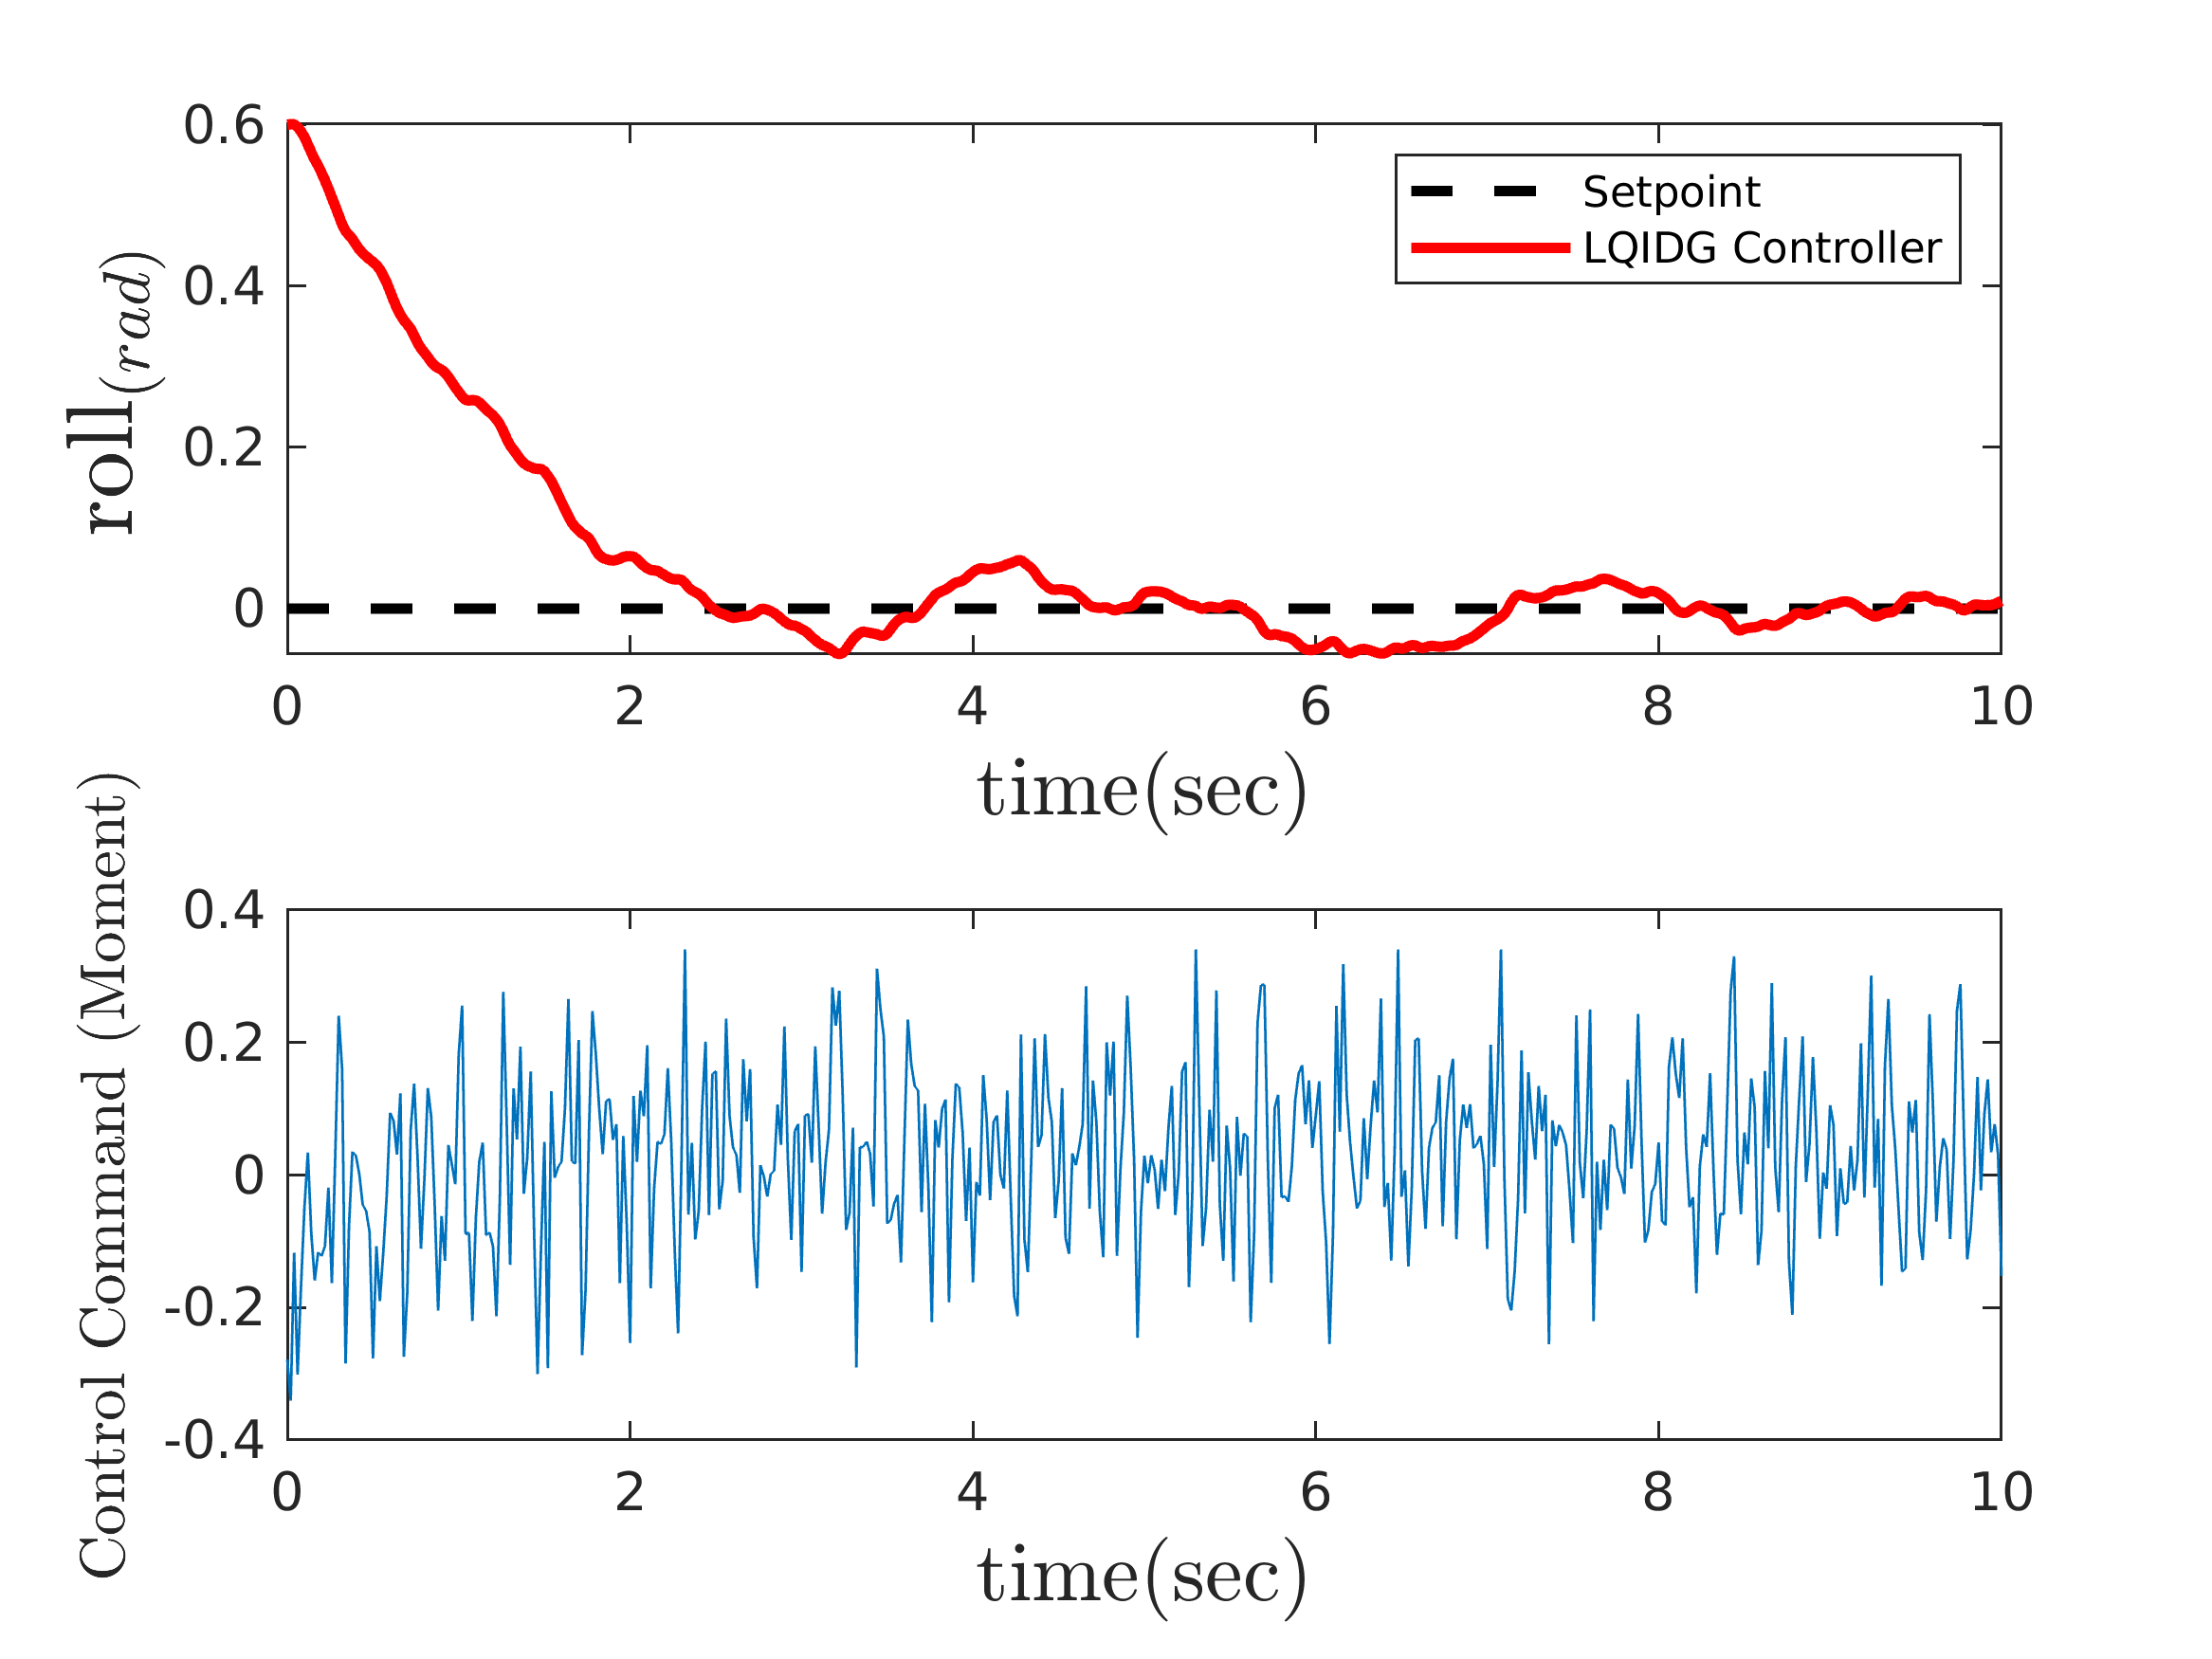
\includegraphics[width=.48\linewidth]{../Figures/MIL/LQIDG/Roll/lqidg_roll.png}
	\centering
	\caption{عملكرد \lr{LQIDG} در کنترل زاويه رول (تعقیب ورودی صفر)}
	\label{lqidg_roll_fig_simulation}
\end{figure}
\begin{figure}[H]
	\centering
	\subfigure[موتور شماره دو]{
		\centering
		\includegraphics[width=.45\linewidth]{../Figures/MIL/LQIDG/Roll/lqidg_roll_Omega_2.png}
	}
	\subfigure[موتور شماره چهار]{
		\centering
		\includegraphics[width=.45\linewidth]{../Figures/MIL/LQIDG/Roll/lqidg_roll_Omega_4.png}
	}
	\caption{‫‪فرمان کنترلی موتورها در کنترل زاویه رول (تعقیب ورودی صفر)}
\end{figure}

بر اساس خروجی شبیه‌سازی (شکل
\ref{lqidg_roll_fig_simulation})
،کانال رول در حضور کنترل‌کننده \lr{LQIDG} در حدود پنج ثانیه به تعادل می‌رسد و خطای ماندگار آن در حدود صفر است.